
La vita di un oggetto è determinata dal suo \textbf{scope}(è un blocco di codice tra parentesi graffe).\newline\newline
A volte ci occorre creare un oggetto che venga \textbf{allocato} nella free memory(heap) e venga \textbf{deallocato} solo quando noi lo vogliamo.\newline\newline
Quindi una variabile che vive indipendente dallo \textbf{scope}
\begin{tcolorbox}[width=\linewidth, boxsep=6pt]
Queste sono le parole \textbf{\code{\textcolor{blue}{chiavi}}} per lavorare sulla \textbf{free memory}:
\lstinputlisting{Capitoli/Allocazione Memoria/Esempi/Key_De_Allocazione.txt}
\end{tcolorbox}

\newpage

\subsection{Key New}
\begin{itemize}
    \item \textcolor{blue}{\code{New}} crea un oggetto sullo \code{heap}
    \item Se la memoria è insufficiente lancerà un eccezione 
    \code{bad\_alloc}
    \item in caso di buona allocazione sarà restituito un \textbf{puntatore} alla locazione di memoria allocata
    \lstinputlisting{Capitoli/Allocazione Memoria/Esempi/EsAllocazioni.txt}
    \item Gli oggetto allocati con \code{\textbf{new}} rimarranno allocati in memoria finché non verranno Deallocati \textbf{esplicitamente}
    \lstinputlisting{Capitoli/Allocazione Memoria/Esempi/EsDeallocazione.txt}
    \item \code{new} un oggetto verrà allocato con la parola \code{new} e sarà richiamato il costruttore della classe(avviene di default anche se non specificato)
\end{itemize}

\subsection{Key Delete}
\begin{itemize}
    \item \textcolor{blue}{\code{delete}} è un operatore che può essere utilizzato solo sui \textbf{puntatori} ritornati da \code{new} oppure su puntatori a null(\code{nullptr})
    \item L'Applicazione di \code{delete} su \code{nullptr} non avrà nessun effetto
    \item Se un oggetto è stato creato con \code{new} esso esiste fino a
    quando non viene esplicitamente distrutto con \code{delete}.
    \item Solo dopo aver usato \code{delete} a quel punto lo spazio in memoria occupato dall’oggetto può venir riutilizzato.
    \item Se \code{delete} viene utilizzata su una \textbf{classe} e in questa \textbf{classe} sarà definito un \textbf{distruttore} allora prima che la memoria venga liberata verrà eseguito il \textbf{distruttore}.
\end{itemize}
\newpage
\subsection{Key Delete[]}
\begin{itemize}
    \item Per liberare lo spazio allocato da una \textcolor{blue}{\code{new}}, sia \textcolor{blue}{\code{delete}} che \textcolor{blue}{\code{delete[]}} devono conoscere la dimensione dell’oggetto
    allocato.
    \item A \textcolor{blue}{\code{delete}} basta conoscere il tipo dell’oggetto puntato(facilmente reperibile).
    \item Ma \textcolor{blue}{\code{delete[]}} deve conoscere anche il numero di
    oggetti puntati.
    \item Quando viene allocata memoria sullo \textbf{heap}, la \textcolor{blue}{\code{new []}} tiene traccia di quanta memoria/numero di elementi
    allocata/i,
    \item di solito salvando l’informazione in un segmento che
    precede immediatamente la memoria allocata.
    \item Ne consegue che un oggetto array allocato mediante
    l’implementazione standard di \textcolor{blue}{\code{new}} occuperà uno spazio
    leggermente superiore del corrispondente statico.
    \item Quanto meno, infatti, lo spazio necessario a contenere la
    dimensione dell’oggetto.
    \begin{tcolorbox}[width=\linewidth, boxsep=6pt]
    \textcolor{red}{\textbf{NB:}} \textcolor{blue}{\textbf{\code{sizeof}}} restituisce solo la grandezza di un \textbf{tipo} specificato \textbf{NON} della memoria fisicamente allocata di una certa istanza. \newline\newline Quindi il calcolo della grandezza di un  tipo di dato avviene alla \textbf{\textcolor{blue}{\code{Compilazione}}} invece il numero di elementi di può sapere solo al tempo di \textbf{\textcolor{blue}{\code{Esecuzione}}}.
    \end{tcolorbox}
    \item Questo vale solo per l’allocazione degli array: in tutti gli
    altri casi viene usato il tipo del puntatore.
\end{itemize}

\subsection{Gestione memoria}
I principali problemi della memoria \textbf{Libera}(Free memory) è:
\begin{itemize}
    \item \textbf{\textcolor{blue}{Ogetti abbandonati(leaked objects)}}: Allocare uno spazio di memoria con \textcolor{blue}{\code{new}} e poi dimenticarsi di usare \textcolor{blue}{\code{delete}} quando non serve più
    \item \textbf{\textcolor{blue}{Cancellazione prematura(Premature deletion)}}: Quando cancelliamo una locazione(\code{delete}) di memoria in modo prematuro. quindi dealloco una porzione di memoria e poi in un altra parte del codice ho un puntatore a questa locazione ormai libera, quindi accendendo a una locazione liberata il comportamento è indefinito.
    \item \textbf{\textcolor{blue}{Doppia cancellazione(Double deletion)}}: Un oggetto deallocato due volte poiché si chiama due volte il suo distruttore.
    
\end{itemize}

\begin{tcolorbox}[width=15cm, boxsep=10pt]
    \textbf{\textcolor{red}{Esempio Cancellazione prematura:}}
    \lstinputlisting{Capitoli/Allocazione Memoria/Esempi/EsbadFreeMem.txt}
    \textcolor{red}{\textbf{NB:}} Perché \textcolor{blue}{\code{p3}} punterà alla stessa locazione di \textcolor{blue}{\code{p2}} ? Questo perché la \textbf{memoria} per allocare oggetti del nostro programma è \textbf{ben precisa}. Si inizia ad \textbf{allocare} dal primo \textbf{indirizzo} fino al ultimo della memoria dedicata al nostro programma. In questo esempio abbiamo allocato un \textcolor{blue}{\code{int}}(che occupa i primi \code{8 bytes}) e subito dopo lo \textbf{de-allochiamo}. quando \textbf{allochiamo} una nuova porzione di memoria cerchiamo uno spazio libero per l'allocazione(che nel nostro deve poter contenere un \textcolor{blue}{\code{char}}) , essendo la \textbf{memoria vuota} lo inserirà a partire dal primo indirizzo delle memoria dedicata al programma. Essendo che \textbf{punterà} proprio a quel indirizzo quando andremo a assegnare un \code{int(999)} sarà valutato come un \textcolor{blue}{\code{char}} ed uscirà \code{þ}(Simbolo associato al codice ASCII).
\end{tcolorbox}
\subsubsection{Problemi: Doppia cancellazione}
\begin{itemize}
    \item Il problema nasce dal fatto che tipicamente il gestore delle
    risorse non è in grado di tenere traccia di quale parte di codice è proprietaria di una risorsa. quindi se faccio una doppia cancellazione io non so quella locazione di memoria effettivamente apparteneva originariamente apparteneva a qualche altra funzione
    \item Quindi il risultato di un doppio \textcolor{blue}{\code{delete}} non è prevedibile
    \lstinputlisting{Capitoli/Allocazione Memoria/Esempi/DoppiaCanc.txt}
    \item Tra il primo e il secondo \textcolor{blue}{delete[]} la memoria può essere stata riutilizzata
\end{itemize}

\subsection{Buone norme d'utilizzo}
\begin{itemize}
    \item Evitiamo di mettere oggetti sullo free store a meno che non
    sia strettamente necessario: meglio usare uno scope il più
    ristretto possibile
    \item Quando un oggetto viene costruito sullo free store, meglio
    inserirlo all’interno di un \textbf{gestore di oggetti} (handle) che
    preveda un distruttore
    \item Come regola pratica: usiamo \textcolor{blue}{\code{new}} dove c’è un costruttore e
    \textcolor{blue}{\code{delete}} dove c’è un distruttore
\end{itemize}

\subsection{Prestazioni}
\begin{itemize}
    \item Una gestione poco attenta dello heap (alternanza di \code{new} e
    \code{delete}) può portare alla sua \textbf{frammentazione}: la
    formazione di buchi nella memoria disponibile.
    \item Questi buchi sono troppo piccoli per poter essere utilizzati
    per allocare nuovi oggetti.
    \item L’effetto è che la memoria che resta disponibile è molto
    meno di quello che ci si aspettava.
    \item Ne consegue anche \textbf{l’aumento dei tempi} di esecuzioni di
    nuovi \code{new}: diventa sempre più difficile andare a cercare
    dove poter mettere il nuovo oggetto.
    \item Cerchiamo di capire come funziona questo meccanismo
    per cercare di prevenirlo
\end{itemize}
\begin{tcolorbox}[width=15cm, boxsep=10pt]
    \lstinputlisting{Capitoli/Allocazione Memoria/Esempi/EsFramenttazione.txt}
    
\end{tcolorbox}
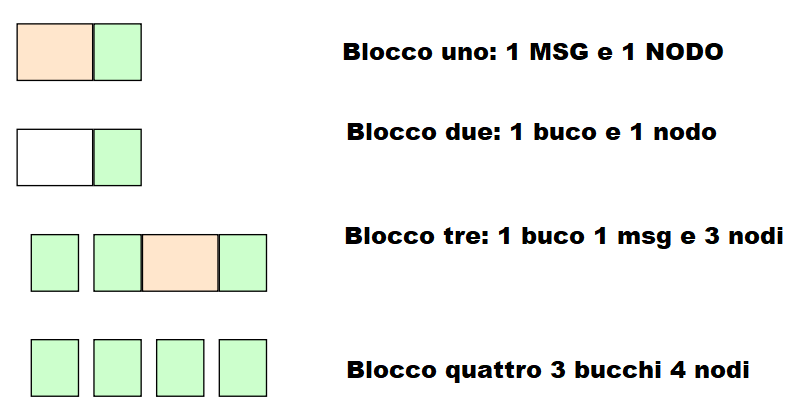
\includegraphics[scale = 0.4]{Capitoli/Allocazione Memoria/Esempi/Blocchi.png}\newline
\begin{itemize}
    \item In questo esempio si vede benissimo che ogni volta che cancello un \  \newline\textcolor{orange}{messaggio} e alloco un nodo si crea un buco poiché il \textcolor{green}{nodo} non è grande quanto la memoria libera creando un buco che non può essere riempito da \newline\textcolor{orange}{messaggio}. reiterando questo blocco di codice avremo sempre piu buchi non utilizzabili
\end{itemize}

\subsection{Soluzioni alla framenttazione}
\begin{itemize}
    \item Due alternative:
    \begin{itemize}
        \item  Un \textbf{garbage collector} per tappare i buchi
        \item  Il programmatore evita di crearli
    \end{itemize}
    \item I puntatori rendono difficile creare un \textbf{garbage collector}
        \begin{itemize}
            \item poiché è difficile spostare le locazioni di memoria al interno della memoria rispetto ad altri linguaggi come \textbf{java} dove si posso spostare gli oggetti al interno della memoria più facilmente 
        \end{itemize}
    \item Come possiamo evitare la formazione dei buchi?
    \item A volte basta riorganizzare la chiamata alle \code{new} e \code{delete}
    \item Ma non è una soluzione generale
    \item \textbf{Prevenire:} evitare usi del free store che provocano
    frammentazione
    \item \textbf{Prima idea:} evitiamo l’uso del \code{delete}, almeno non
    rallentiamo nuovi \code{new}, almeno nella maggior parte delle
    implementazioni, anche se non è garantito dallo standard.
    \item \textbf{Seconda idea:} allochiamo tutta la memoria (statica e
    globale) all’inizio del programma e poi la usiamo.\newline\newline
    \textcolor{blue}{\textbf{Svantaggi:}} struttura del programma non ottimale e uso di
    dati globali da evitare.
\item Due \textbf{strutture} dati possono \textbf{aiutarci} in questo:
    \begin{itemize}
        \item  \textcolor{blue}{\textbf{Stack}} : visto che si allunga e si accorcia solo da una
        parte non può causare frammentazione
        \item \textcolor{blue}{\textbf{Pool}} : una raccolta di oggetti della stessa
        dimensione. Essendo della stessa
        dimensione, non può esserci frammentazione.
    \end{itemize}
    \item Con entrambe queste soluzioni, sia \textbf{l’allocazione} che la
    \textbf{deallocazione} hanno tempi prevedibili e veloci.
    Se non si gestisce la frammentazione potremo avere tempi lunghi di allocazione e non prevedibili
\end{itemize}
